% Autor: Alfredo Sánchez Alberca (email:asalber@ceu.es)
% Charts that shows the purpose of Statistics
\begin{tikzpicture}[every label/.style={text=color1}]
\tikzstyle{node} = [align=center, node distance=1cm, text=color1]; 
\tikzstyle{arrow} = [-latex, color1, line width=10pt];

\node (data) [label=-90:Datos] at (0,1) {
\includegraphics[height=1.5cm]{img/introduccion/datos.pdf}}; 
\pause
\node (information) [label=-90:Información] at (4.7,1)
{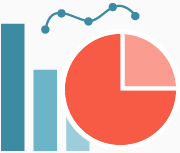
\includegraphics[height=1.5cm]{img/introduccion/informacion.png}}; 
\node at (2,1) [fill=color1,single arrow,shape border rotate=0,text=white, minimum width=1.1cm]{
\ ESTADÍSTICA\ \phantom{}};
\pause
\node (knowledge) [label=-90:Conocimiento] at (9.5,1) {
\includegraphics[height=1.5cm]{img/introduccion/conocimiento.png}};
\node at (7,1) [fill=color1,single arrow,shape border rotate=0,text=white, minimum width=1.1cm]{
Interpretación\phantom{}};
\pause
\node at (11.5,1) [fill=color1,single arrow,shape border rotate=0,text=white, minimum width=1.1cm]{
\ Decisiones\ \phantom{}};
\end{tikzpicture} 